%%%%%%%%%%%%%%%%%%%%%%%%%%%%%%%%%%%%%%%%%%%%%%%%%%%%%%%%%%%%%%%%%%%
%                                                                 %
%  GEANT manual in LaTeX form                                     %
%                                                                 %
%  Michel Goossens (for translation into LaTeX)                   %
%  Version 1.00                                                   %
%  Last Mod. Jan 24 1991  1300   MG + IB                          %
%                                                                 %
%%%%%%%%%%%%%%%%%%%%%%%%%%%%%%%%%%%%%%%%%%%%%%%%%%%%%%%%%%%%%%%%%%%  
\Origin{P.Zanarini}
\Documentation{P.Zanarini, F.Carminati}
\Submitted {01.01.86}   \Revised{11.12.92}
\Version{Geant 3.15}\Routid{DRAW115}
\Makehead{Drawing a Volume Projection view -- Case 2}
\Shubr{GDRVOL}{(NNAMS,CHNAMS,LNUMBS,NRS,THETA,PHI,PSI,U0,V0,SU,SV)}
Draws an orthographic parallel projection or a perspective projection 
(depending on the option chosen via \Rind{GDOPT}) of the volume 
{\tt CHNAMS(N),LNUMBS(N)} with all its descendants, at the position 
{\tt U0,V0} (user coordinates), with the scale factors {\tt SU} and 
{\tt SV}. 
The object is seen from {\tt THETA} and {\tt PHI} angles, 
and the resulting 2D projection is also rotated by an angle {\tt PSI} 
on the screen plane. These parameters, as well as zoom parameters set 
by \Rind{GDZOOM}, define the current {\it view parameters}, and they are 
copied in \FCind{/GCDRAW/}.  Attributes like colour, fill area, line 
width, line style, visibility, etc. can be set by the \Rind{GSATT} 
routine for {\tt CHNAMS(N)} and or its descendants {\tt [GEOM 500]}.
This routine differs from \Rind{GDRAW} in the following aspects:
\begin{itemize}
\item  The object to be drawn is identified by a full path. This gives 
the possibility of drawing a particular copy or division of a volume, or 
even a volume that has more than one mother in the geometry tree.
{\tt CHNAMS(1),...,CHNAMS(N)} contain the volume names and
{\tt LNUMBS(1),...,LNUMBS(N)}, the volume numbers defining the path 
to go from the top volume to the one to be drawn.
\item  The object can be drawn either with respect to the
{\tt MA}ster {\tt R}eference {\tt S}ystem ({\tt NRS=0}) or with respect 
to its {\tt D}augther {\tt R}eference {\tt S}ystem (i.e. the Local R.S.); 
in the first case it is drawn in its position in the real world, while 
in the second one it is drawn like \Rind{GDRAW} would do.
\item  In this latter case, track and hit points will be
drawn with respect to the {\tt DRS} of the volume last
drawn by this routine, and not with respect to the
{\tt MARS} as is done normally (to reset to the normal
case a call with {\tt NRS=0} or {\tt NNAMS=0} is required).
\end{itemize}
\begin{DLtt}{MMMMMM}
\item[NNAMS]     ({\tt INTEGER}) number of elements {\tt levels} in the 
arrays {\tt CHNAMS, LNUMBS}. The bottom volume of this path is also the 
one that is actually drawn;
\item[CHNAMS]   ({\tt CHARACTER*4}) array of volume name (dimensioned 
at least to {\tt NNAMS});
\item[LNUMBS]   array of volume numbers (dimensioned at least to {\tt NNAMS});
\item[NRS]    reference system used:
\begin{DLtt}{MMMMM}
\item[NRS$=$0] to have the volume(s) drawn with respect to the {\tt MARS} 
\item[NRS$\neq$0] to have the volume(s) drawn with respect to the {\tt DRS}
\end{DLtt}
\item[THETA]   $\theta$ angle between the line of sight and the
                Z  axis of {\tt MARS};
\item[PHI]    $\phi$ angle between the projection of the line of sight
              on plane {\tt X Y} and the {\tt X} axis of {\tt MARS}
\item[PSI]   $\psi$ angle by which the projected image will
             be rotated on the screen plane
\item[U0]    u coordinate on the screen of the volume origin
\item[V0]    v  coordinate on the screen of the volume origin
\item[SU]   scale factor for u coordinates
\item[SV]   scale factor for v coordinates
\end{DLtt}
 
Two examples of use of \Rind{GDRVOL} are shown in fig~\ref{fg:draw115-1} and
\ref{fg:draw115-2}.

\begin{figure}[hbt]
      \centering
      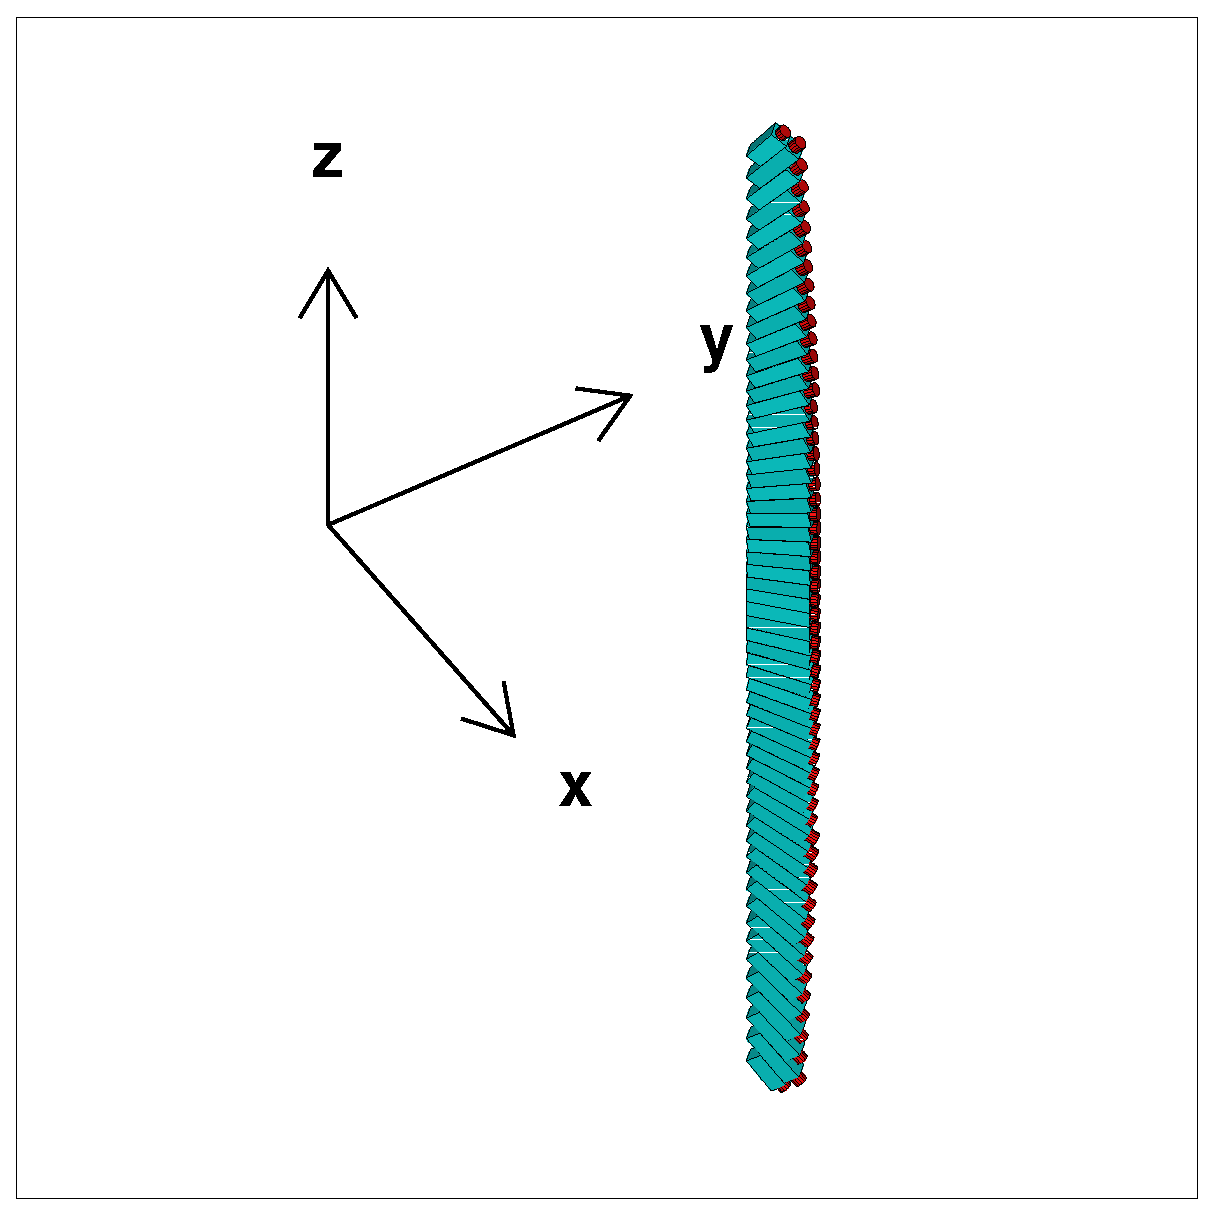
\epsfig{file=eps/draw115-1.eps,width=12cm}

\begin{verbatim}
       CHARACTER*4 CHNAMS(5)
       INTEGER LNUMBS(5)
       DATA CHNAMS/'OPAL','BRL-','EB  ','EBB ','EBP '/
       DATA LNUMBS/    1 ,    1 ,    1 ,    1 ,   20 /
       .
       .
       .
       NRS=0
       CALL GDRVOL(5,CHNAMS,LNUMBS,NRS,80.,135.,0.,13.,10.,0.03,0.03)
       CALL GDAXIS(0.,0.,0.,200.)
C      CALL GDXYZ(0)
\end{verbatim}

     \caption{Example of use of {\tt GDRVOL} in the MAster Reference System}
     \label{fg:draw115-1}


\end{figure}


\begin{figure}[hbt]
     \centering
     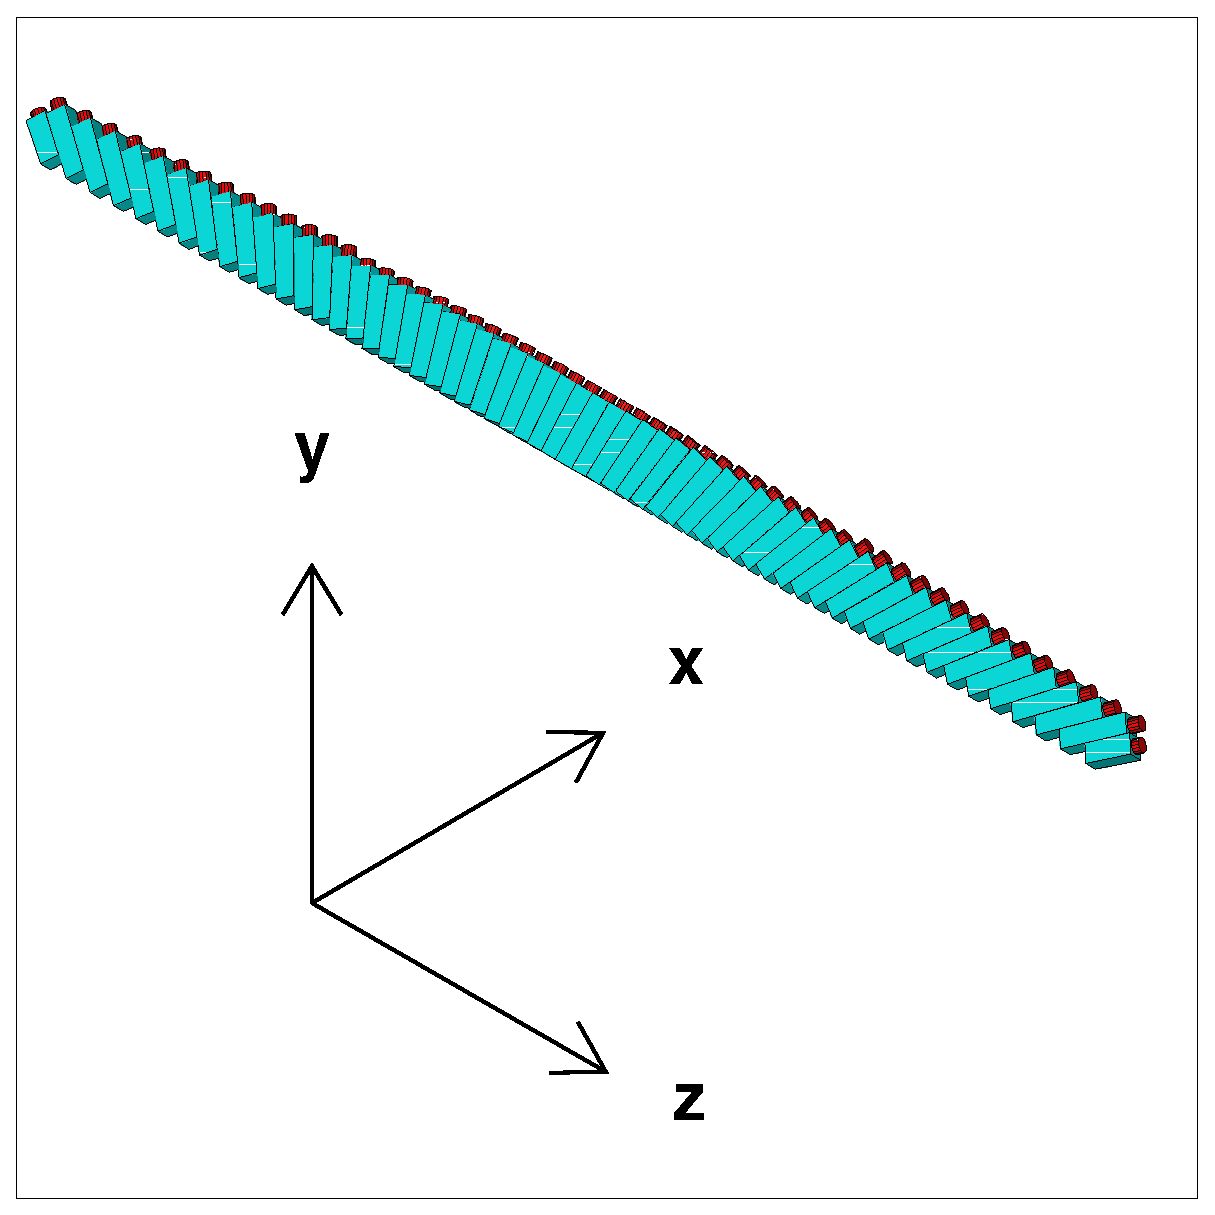
\epsfig{file=eps/draw115-2.eps,width=12cm}

\begin{verbatim}
      CHARACTER*4 CHNAMS(5)
      INTEGER LNUMBS(5)
      DATA CHNAMS/'OPAL','BRL-','EB  ','EBB ','EBP '/
      DATA LNUMBS/    1 ,    1 ,    1 ,    1 ,   20 /
      .
      .
      .
      NRS=1
      CALL GDRVOL(5,CHNAMS,LNUMBS,NRS,55.,135.,0.,5.,5.,0.035,0.035)
      CALL GDAXIS(0.,0.,0.,200.)
C     CALL GDXYZ(0)
\end{verbatim}

\caption{Example of use of {\tt GDRVOL} in the Daughter Reference System}
\label{fg:draw115-2}
\end{figure}
 
